% !TeX root = ../presentation.tex

\section{Project}
\begin{frame}{Initial situation}
	\setbeamercovered{transparent}
	\begin{itemize}
		\item<1-> Use openSenseMap
		\item<2-> Get urban temperature sensors for Berlin
		\item<3-> Interpolate data using different methods 
		\item<4-> Create animation
		\item<5-> Compare results
	\end{itemize}
	\setbeamercovered{invisible}
\end{frame}
\begin{frame}{Problems: Getting the data}
\begin{columns}[c] % align columns
	\begin{column}{.52\textwidth}
		\begin{itemize}
			\item openSenseMap offers API access
			\item For bbox sensor data a phenomenon name must be given
			\item Phenomenon/Sensor name is a free-text field
			\item Different notations
			\item<2-> Most common one (Temperatur) was chosen
		\end{itemize}
	\end{column}%
	\hfill%
	\begin{column}{.48\textwidth}
		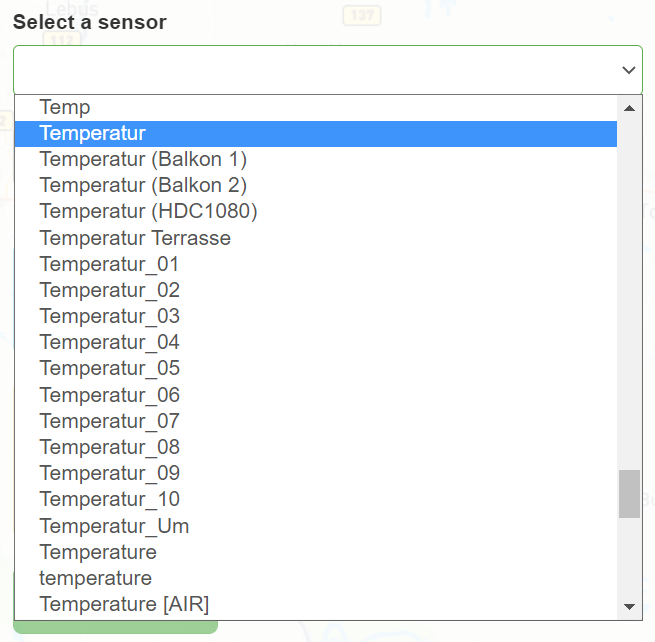
\includegraphics[width=\linewidth]{../writeup/images/phenomenon_name.png}
	\end{column}%
\end{columns}
\end{frame}
\begin{frame}{Problems: Aggregating data}
	\begin{itemize}
		\item Aggregated export does not cover full day
		\item Raw data may not include measurements throughout the day
		\item<2-> Manually aggregate raw data into 10 minute averages
		\item<2-> Filter out all stations that didn't provide measurements for every 10 minute interval
	\end{itemize}
\end{frame}
\begin{frame}{Problems: Data quality}
\begin{columns}[c] % align columns
	\begin{column}{.55\textwidth}
		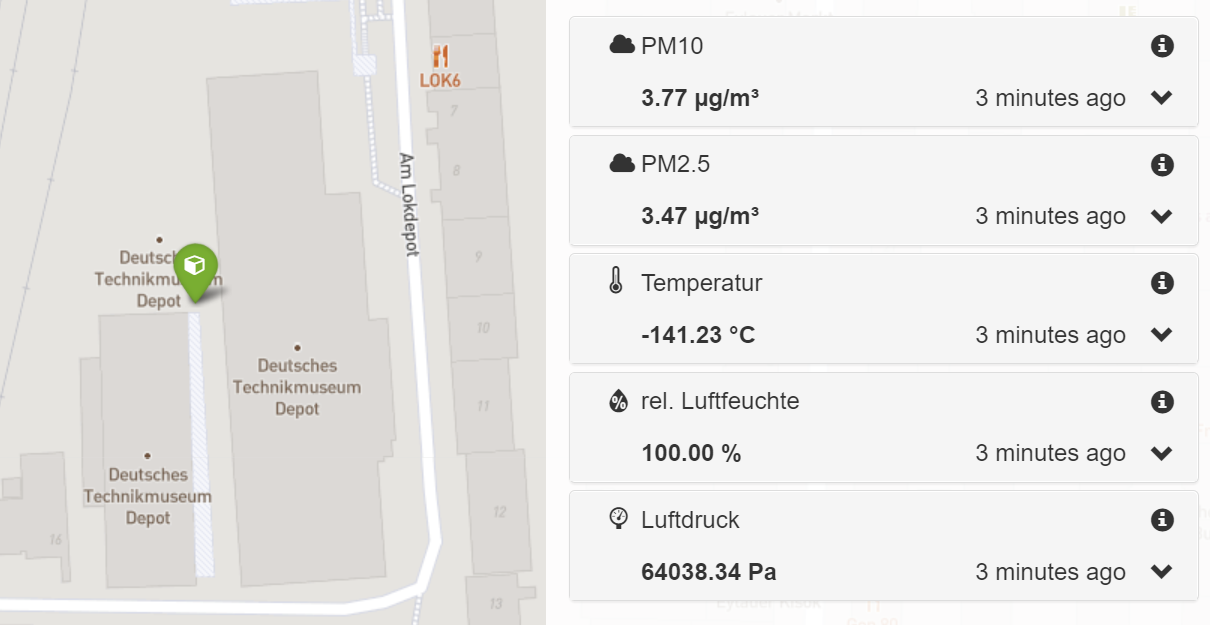
\includegraphics[width=\linewidth]{../writeup/images/outliers.png}
	\end{column}%
	\hfill%
	\begin{column}{.45\textwidth}
		\begin{itemize}
			\item Citizen-science project
			\item No validation of submitted data
			\item Do you spot any issues with the measurements?
			\item<2-> Filter all measurements that are more than double standard deviation from mean
		\end{itemize}
	\end{column}%
\end{columns}
\end{frame}
\begin{frame}{Final Workflow}
	\centering
	\scalebox{0.85}{
		\begin{tikzpicture}[node distance = 2cm, auto, every node/.style={color=text, fill=background, font=\sffamily}, align=center]
			% Place nodes
			\node [block] (in) {openSenseMap};
			\node [cloud, right=1.6cm of in, text width=7em] (avg) {Average\\into 10 minute intervals};
			\node [cloud, right=1.6cm of avg, text width=8em] (filter) {Filter\\by std deviation};
			\node [decision, below=1.6cm of filter] (interpolate) {Interpolate};
			\node [cloud, left=1.6cm of interpolate, text width=8em] (colorize) {Colorize\\1-band Tiff $\Rightarrow$ 4-band RGBA Tiff};
			\node [block, below=2.3cm of in] (out) {Generate frame};
			% Draw edges
			\draw [->] (in) -- (avg);
			\draw [->] (avg) -- (filter);
			\draw [->] (filter) -- (interpolate);
			\draw [->] (interpolate) -- (colorize);
			\draw [->] (colorize) -- (out);
		\end{tikzpicture}
	}
\end{frame}